% SLIDE
\begin{frame}
	\frametitle{Shifting the trust anchor}
	\begin{itemize}
		\item Server is the authoritative source of match state: the client cannot tamper with it
		\item Analyze gameplay telemetry the server already receives, instead of inspecting the client
		\item No privileged access to the player's machine required
	\end{itemize}
\end{frame}

% SLIDE
\begin{frame}
	\frametitle{Pipeline architecture}
	\begin{itemize}
		\item Threshold scorer: 8 flags (time-to-damage, headshot ratio, reaction time, etc)
		\item LSTM scorer: tracks anomaly consistency across rounds and matches
		\item Suspicion score: weighted combination $\Rightarrow$ human review
	\end{itemize}
	\begin{center}
		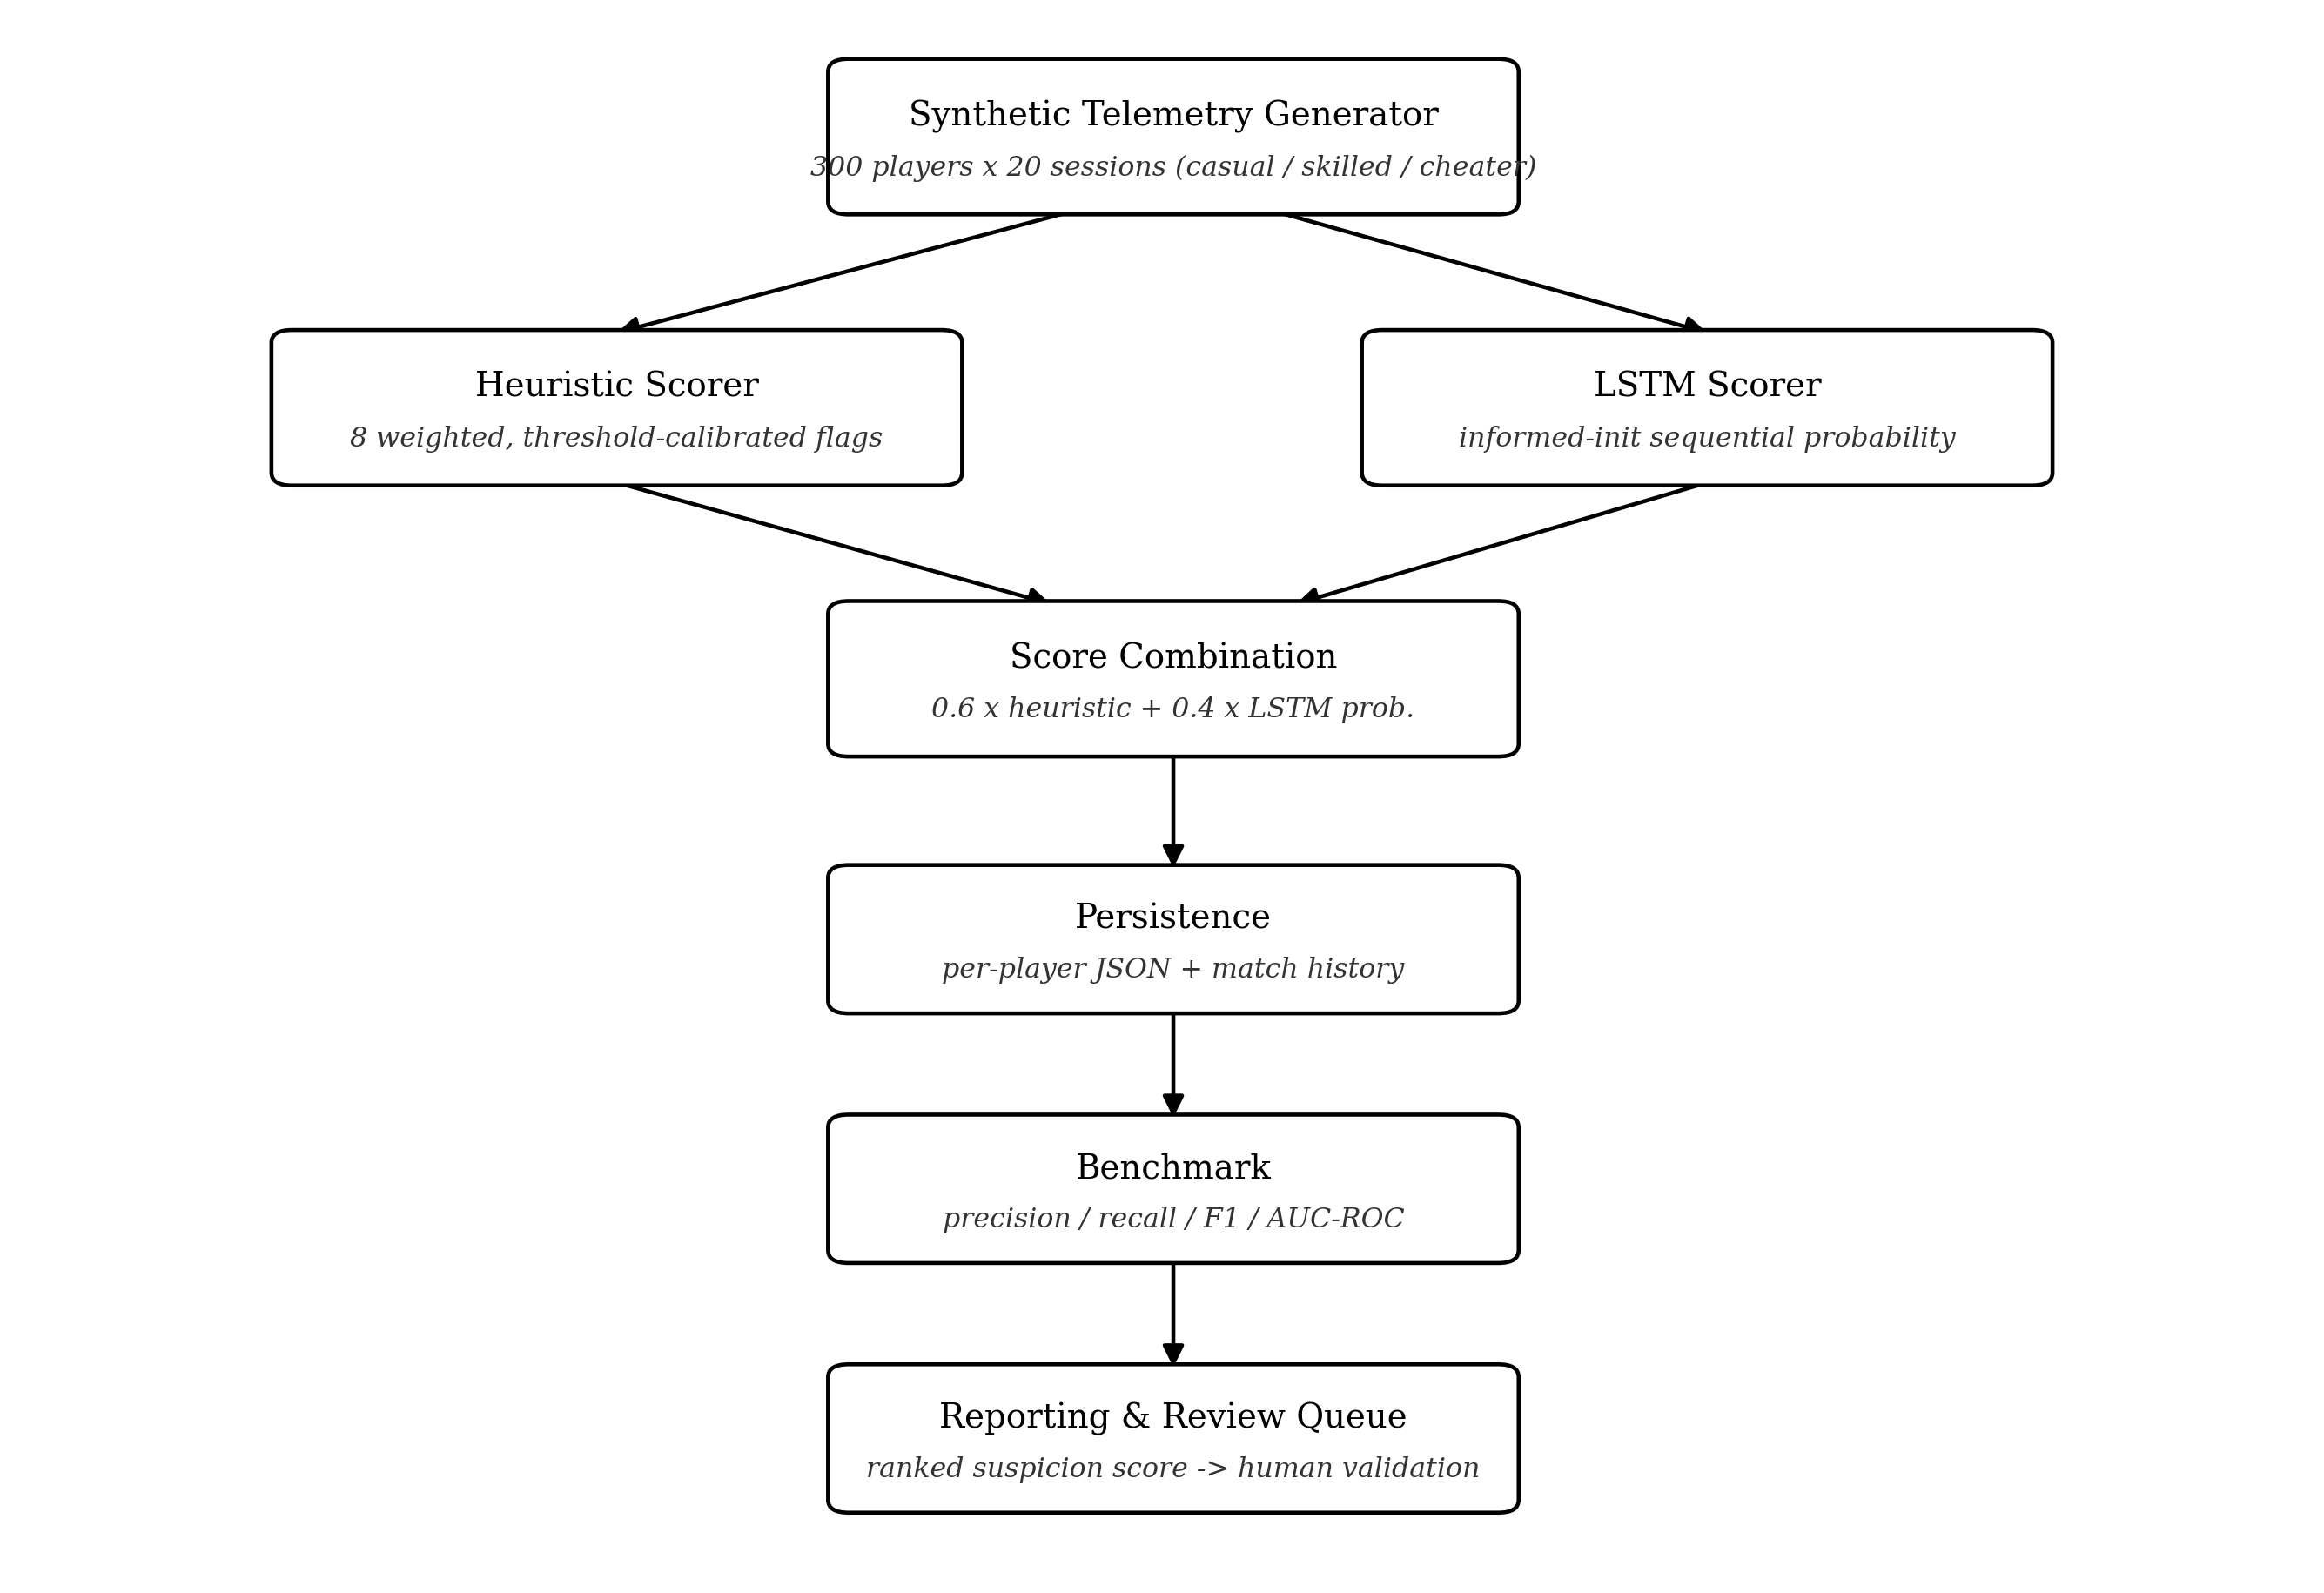
\includegraphics[height=4.5cm]{../images/chap03/pipeline_diagram.png}
	\end{center}
\end{frame}

% SLIDE
\begin{frame}
	\frametitle{Dataset design and the high-skill bias}
	\begin{itemize}
		\item Synthetic dataset: 300 players with casual / skilled / cheater profiles
		\item Calibrated from online benchmarks and personal experience
		\item Challenge: elite players can statistically resemble subtle cheaters
		\item Distributions deliberately overlapped around that boundary to empathize the hardest case
	\end{itemize}
	\begin{center}
		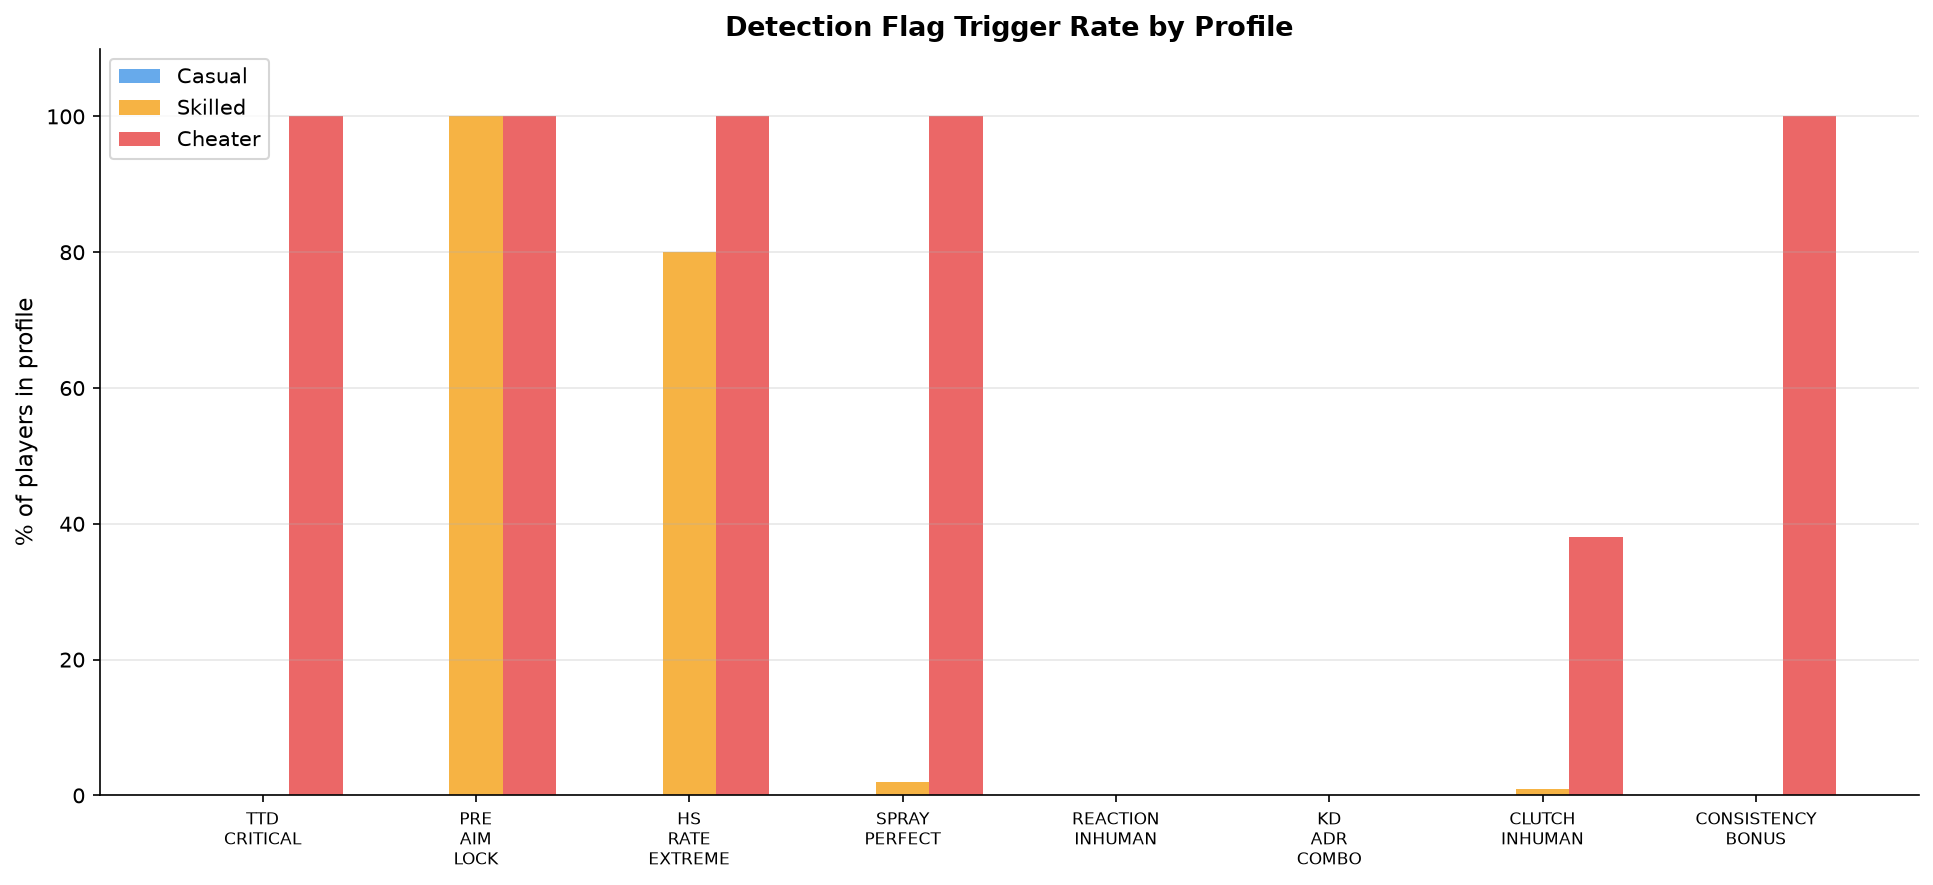
\includegraphics[height=3.5cm]{../images/chap03/flag_frequency.png}
	\end{center}
\end{frame}

% SLIDE
\begin{frame}
	\frametitle{Results}
	\begin{itemize}
		\item Clear statistical separation between legitimate players and cheaters at the population level
		\item \bf 0\% false positives on legitimate players, 51\% of cheaters correctly flagged
	\end{itemize}
	\begin{center}
		\begin{minipage}{0.48\textwidth}
			\centering
			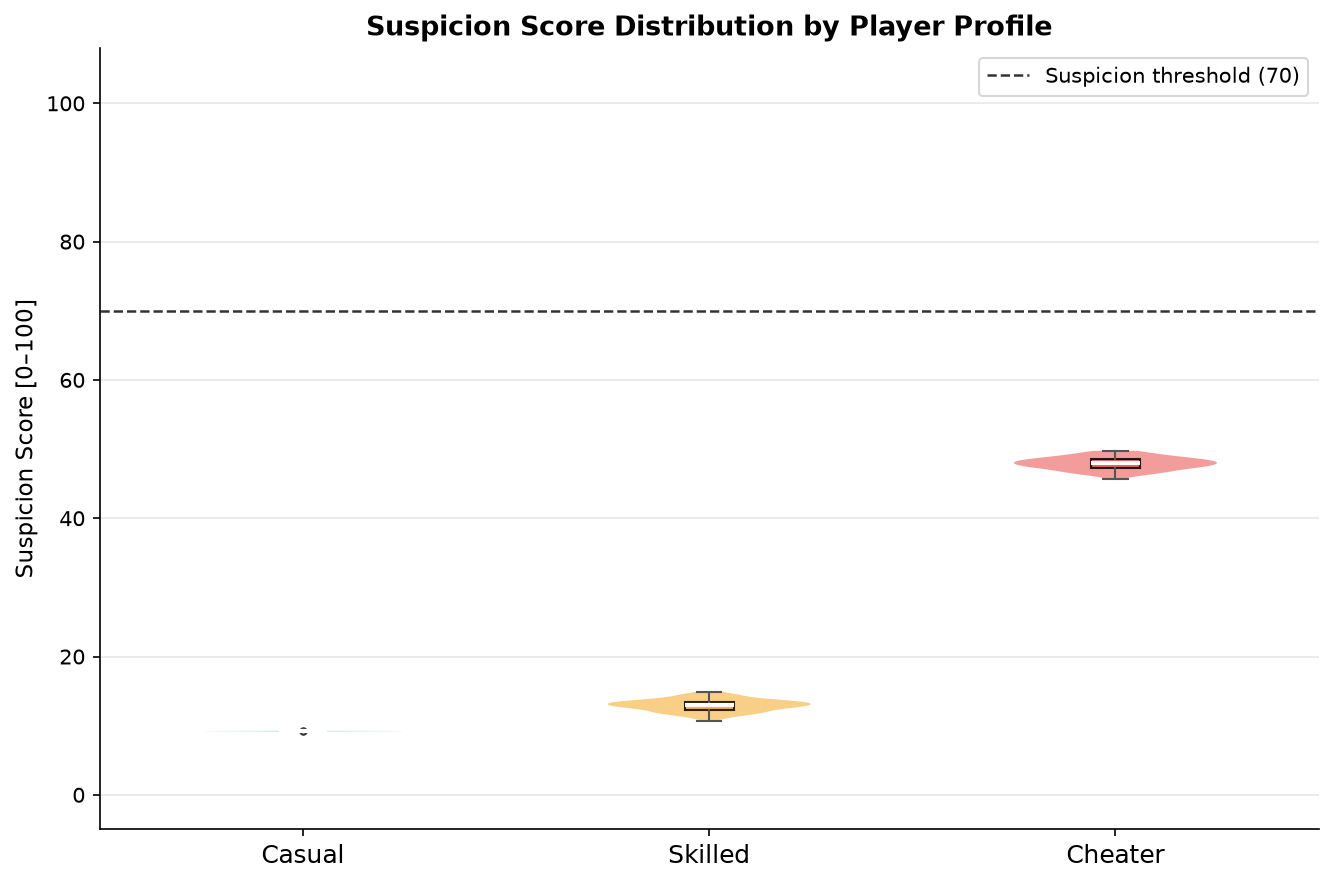
\includegraphics[height=3.75cm]{../images/chap03/score_distribution.png}
		\end{minipage}
		\hfill
		\begin{minipage}{0.48\textwidth}
			\centering
			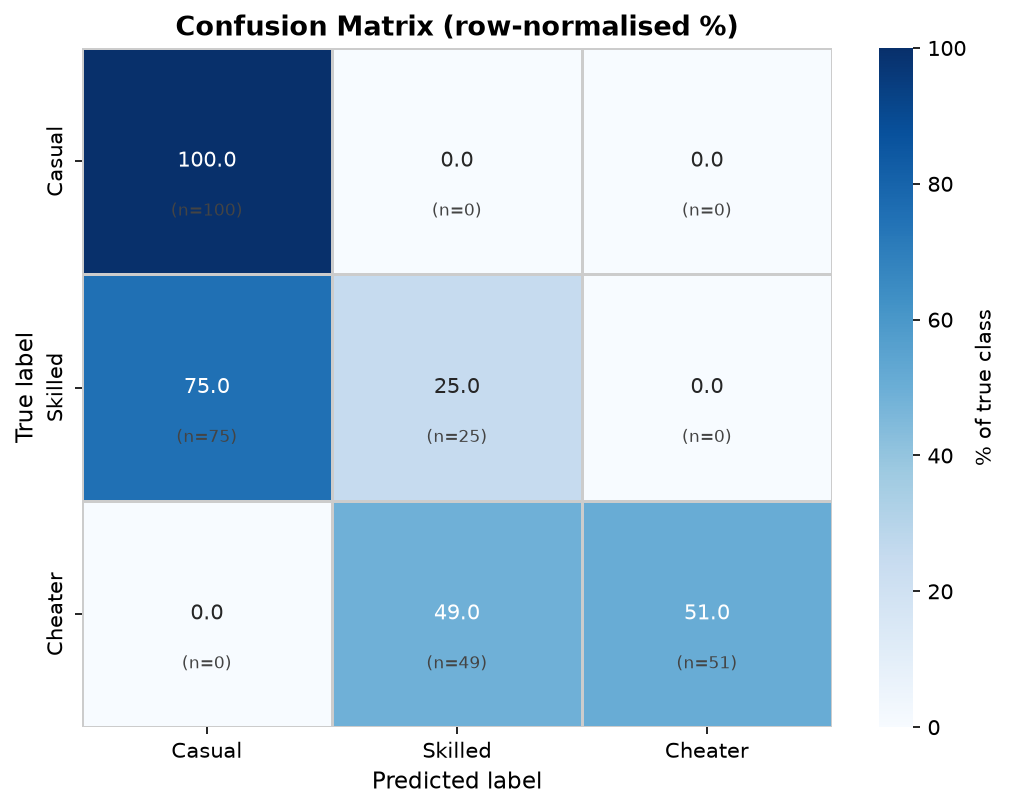
\includegraphics[height=3.75cm]{../images/chap03/confusion_matrix.png}
		\end{minipage}
	\end{center}
\end{frame}
